\documentclass[tikz,border=10pt]{standalone}
\usepackage{amsmath}
\usetikzlibrary{angles,quotes}
\begin{document}
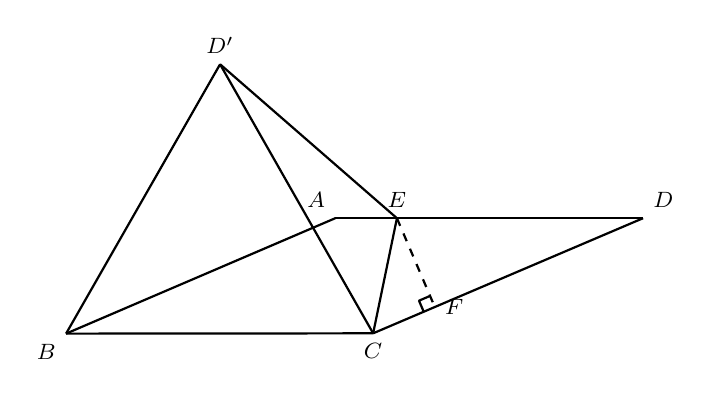
\begin{tikzpicture}[line width=0.8pt, line join=round]
\coordinate (A) at (-0.260,-0.248);
\coordinate (B) at (-3.679,-1.714);
\coordinate (C) at (0.221,-1.710);
\coordinate (D) at (3.649,-0.248);
\coordinate (E) at (0.523,-0.248);
\coordinate (F) at (1.004,-1.376);




\coordinate (Dp) at (-1.723,1.707);


\draw (A) -- (B);
\draw (A) -- (E);
\draw (E) -- (D);

\draw (C) -- (F) -- (D);
\draw (Dp) -- (C);
\draw (Dp) -- (E);
\draw (Dp) -- (B);
\draw (B) -- (C);
\draw (E) -- (C);


\draw[dashed] (E) -- (F);


\draw pic[draw, angle radius=0.153cm] {right angle=C--F--E};


\node[above left] at (A) {\fontsize{8}{9.6}\selectfont $A$};
\node[below left] at (B) {\fontsize{8}{9.6}\selectfont $B$};
\node[below] at (C) {\fontsize{8}{9.6}\selectfont $C$};
\node[above right] at (D) {\fontsize{8}{9.6}\selectfont $D$};
\node[above] at (E) {\fontsize{8}{9.6}\selectfont $E$};
\node[right] at (F) {\fontsize{8}{9.6}\selectfont $F$};
\node[above] at (Dp) {\fontsize{8}{9.6}\selectfont $D'$};
\end{tikzpicture}
\end{document}